\documentclass[12pt]{report}
\usepackage[utf8]{inputenc}
\usepackage{graphicx}
\usepackage{hyperref}
\usepackage{setspace}
\usepackage[export]{adjustbox}
\usepackage{tikz}
\usepackage[titletoc]{appendix}
\usepackage{hyperref}
\hypersetup{hidelinks}

\usepackage{graphicx}
\usepackage[export]{adjustbox}
\setstretch{1.4}
\usepackage{geometry}

\title{
	%Institution Logo	
	\begin{tikzpicture}[remember picture,overlay]
	   \node[anchor=north east,inner sep=70pt] at (current page.north east)
	              {
\includegraphics[height = 3cm]{kcllogo.jpg}};
	\end{tikzpicture}
		
	%Actual Title
	\textbf{\LARGE{An Intelligent Tutoring System for First-Year Level Java}}
	
	%Degree
	\vspace{0.9cm}
	\large{6CCS3PRJ Final Project: Final Report Submission}\\[-1.5ex]
	\vspace{0.9cm}
	\large{BSc Computer Science with a Year in Industry}
	
	%Student and Supervisor
	\large{Author: Miruna-Ioana P\^irvulescu}\\[-1ex]
	\large{Supervised by: Dr. Sahar Al-Sudani}\\[-1ex]
	\large{Student Number: 1701543}\\ [-1ex]
}

\begin{document}
	%Title Page
	\maketitle
	
	%Originality Avowal
	\begin{center}
		\textbf{\large{Originality Avowal}}
	\end{center}
	\emph{I verify that I am the sole author of this report, except where explicitly stated to the contrary.}
	\begin{flushright}
		Signature: \emph{Miruna-Ioana P\^irvulescu}\\
		Date: \today
	\end{flushright}
	
	%Abstract
	\newpage
	\begin{center}
		\textbf{\large{Abstract}}
	\end{center}
	
	%About education
	The present day is relying more and more on the use of technology, and the education sector is no exception. An increasing number of schools is opting for smart pedagogical solutions in their classrooms through the use of specialised hardware (such as smart boards) and software applications (for example, learning management systems).\\

	%About the project
	This project aims to implement a simple Intelligent Tutoring System meant to teach first-year university students in Computer Science how to code in Java. The implemented solution is a piece of software that queries and infers details from an ontology that encapsulates the topic. The application is able to provide information about Java statements, types, operations, and object orientation.
	
	
	%Acknowledgements
	\newpage
	\begin{center}
		\textbf{\large{Acknowledgements}}
	\end{center}

	%To Dr. Al-Sudani
	I would like to thank Dr. Al-Sudani for all the guidance, feedback, and support offered throughout the development of this project. I found our meetings to be very helpful in choosing the best approaches that led to the creation of this application.\\\\

    %To the university
    Many thanks to the Department of Informatics for the quality of the modules taught throughout this degree. All the knowledge I accrued over the past four years has enabled me greatly to produce this project.\\\\

    %To the testers
    I would also like to thank everybody who provided feedback during the evaluation stage of the project from the point of view of the end user.

	%Contents
	\newpage
	\tableofcontents

	%Introduction
	\chapter{Introduction}

	%Motivation
	\section{Motivation}
	The biggest exposure that a Computer Science student has to cutting-edge technologies comes from their personal rather than academic environments, through video games, streaming applications, or social media. The academic curriculum is mostly theory-based and human-taught, with some components of programming assignments and classroom examples that are only lightly explained.
    \newline
    This traditional method is a very effective and informative approach to teaching. However, it is lacking an engagement factor of practical demonstration. This factor could potentially drive students to seek further information on their course topics and to achieve better results from their learning, meaning that they are exploiting their academic resources to the largest extent.
    \newline
    This project is meant as a step forward in smarter education. By developing a well-rounded knowledge formalism and creating a small application to display its information to users, student engagement has the potential to rise through exposure to a modern teaching style. Rather than having a human explain a type of technology, that technology can ``gain a voice'' and teach the student about itself.

	%Key terms
	\section{Three Key Terms}
	An \textbf{Intelligent Tutoring System} (ITS) is a type of software application aimed at teaching students about various topics, requiring little to no intervention from a human expert \cite{itsdefinition}.\\
    A \textbf{Domain Model} refers to the knowledge that the ITS uses to produce human-readable data through referencing given knowledge and inferring new facts.
    \\
    The most important term of this project is the \textbf{ontology}. In the field of Computer Science, an ontology is a method of representing entities in rapport to one another through means of relations. For example, the class Car \emph{is} a sub-category of the class Vehicle and it \emph{has} multiple Wheels that allow it to move.
	
	%Project Aims
	\section{Aims and Objectives}
	The first objective of the project is to create a basic Intelligent Tutoring System. This system aims to teach first-year Computer Science undergraduate students about programming in Java. The main topic is looking at different statement types, such as Conditional and Loop Statements.
	\newline
	The second objective of the project is to build a Domain Model as a computer-readable formalism, such as an ontology. The system must be able to make inferences based on this formalism. Moreover, it must present all the domain-specific information, both given and inferred, to the end user.
	\newline
	The application must be intelligible, informative, engaging, and easy to use.
	\newline
	For the purpose of this project, a research component was essential in order to understand how such a system can be developed. Chapter 2 will explore this research in detail.
	
	%Background
	\chapter{Background}
	This chapter covers an extended overview of the key terms described above, as well as thorough descriptions of the research items that shaped the final software. The chapter also includes technology comparisons and literature reviews to describe the thought process behind the software structure.
	
	%What is an ITS
	\section{Intelligent Tutoring Systems}
	As previously defined, an Intelligent Tutoring System is a type of application that can teach a subject to students without need for additional, human support. Such a system is constructed based on four pillars, called \emph{models}.\\
	First, an ITS has a \emph{Student Model}. This is meant to track the progress made by the learner throughout their studies and offer corrections where necessary.\\
	Secondly, the Intelligent Tutoring System has a \emph{Pedagogical Model}. Its purpose is to identify an optimal teaching strategy based on the learning style of the student.\\
	The third pillar is called the \emph{User Interface Model}. This enables the student to access the knowledge behind the ITS through a Graphical User Interface. In the context of this project, this is represented by the front end of the web application.\\
	Finally, an Intelligent Tutoring System has a \emph{Domain Model}. This is also known as the knowledge model, and it is represented by a knowledge representation formalism.\\
    The main focus of this project is the implementation of the Domain Model. Therefore, its implementation is the vital component of the software. The following sections describe how this model has been implemented and why were the used technologies chosen.
	
	%KRF
	\section{Knowledge Representation Formalisms}
	Knowledge representation formalisms are means of expressing the human-readable information in a computer-readable fashion. Some examples of such formalisms are ontologies, semantic networks, frames, and rule-based systems.\\
	The process of deciding which of these types of formalisms better suits this project involved significant research, comparisons between findings, and a small component of personal preference.
	
	%ontologies
	\subsection{Ontologies}
    Ontologies encapsulate the formal design and definition of a class hierarchy. They are widely used within the field of education \cite{wikiontology}, as well as in knowledge representation and design. Due to the rigorous hierarchical nature of ontologies, their use became best candidate for the development of this project.\\
    As defined in Chapter 1, ontologies represent entities (or classes) and relations (more commonly known as properties) between these. Properties have various restriction types, and the easiest one to exemplify is restriction \emph{is}. This simply implies that an entity is a subclass of another entity. For example, class Pet \emph{is} (commonly) a subclass of entity Animal. Other relations can be defined. For example, a Pet \emph{sleeps} in a Bed (where Pet and Bed represent different classes).\\
  
    %%%%%%%%%%%%%%%%
    % Move to Body %
    %%%%%%%%%%%%%%%%
    In ontologies, the classes involved in a property are similar to the sets in a mathematical function. In mathematics, the expression \(f: A \rightarrow B, f(x) = y\) means that function f maps element x of the \emph{domain} (that is, set A) to element y of the \emph{codomain} (set B). Similarly, in ontology properties, a class becomes a domain, and the other class is the codomain. A small yet important difference is that ontologies refer to the codomain as the \emph{range} of a property. The same expression can be re-written in the previous example as: \[sleeps: Pet \rightarrow Bed, sleeps(pet\_x) = bed\_y\]
    This means that, for the \emph{sleeps} property, the class Pet is the domain, and class Bed is the range.\\
    Before detailing more about properties, the notion of \emph{instance} needs to be introduced. An instance is a specific element belonging to a class. For example, class Pet can have instances Pet\_Bed and Human\_Bed.
    \\
    Apart form the subclass/superclass property restriction \emph{is}, this project uses another two kinds of relations. These are the \emph{has-value} and \emph{some-value} relations.\\
    The two types of restrictions are similar in the sense that they allow two classes to connect a domain to a range. The differences are quite significant however, and that is why they were both necessary in building the ontology for the project.\\
    Some-value restrictions represent class-to-class connections. For example, a some-value restriction would allow a Pet to sleep in Bed, not only in their own.\\
    Has-value restrictions are more severe. They only allow class-to-instance properties. For example, a Pet can only sleep in their Bed, and not sleep in any other Bed.\\
    

    %semantic nets
    \subsection{Semantic Networks}
    Semantic networks are visually represented by graphs, where the entities are the vertices and the relations are the edges \cite{semnet}. They share a lot of similarities with ontologies, however semantic networks are less rigorous formalisms. \cite{semnetvsonto}
    \newline
    Because of this, only the graphical representation of semantic networks has been used for the initial structuring of the knowledge model. The first data diagrams were created in the form of mind maps, which perfectly resemble the visual component brought by semantic networks. (An example of such a mind map will be provided in the Development section.)

    %frames
    \subsection{Frames}
    Frames are very widely used for knowledge modelling in Artificial Intelligence. They make use of smaller ontologies that are interconnected to generate the bigger picture.
    \newline
    This type of formalism is a better fit for larger scopes than the one of this project's domain, and therefore its usage would have brought a risk of increasing the complexity of the project above necessity. However, for the description of a larger variant of this domain, where the model would have to also cover various APIs of Java or more in-depth object oriented practices, frames would have been a perfect fit.
    
    %rule base
    \subsection{Rule-Based Systems}
    As the name suggests, a rule-based system is a set of rules (if-else statements). These rules are used to teach the expert system about the domain and how to infer new information from it. This is the classic method of creating expert systems.
    \newline
    While rule-based systems are very strong competitors for ontologies, a general comparison study between the two suggests that rule-based systems are less descriptive than their adversary \cite{rulesvsonto}.
    
    %conclusions on comparison
    \subsection{Final Notes}
    While all the assessed knowledge representation formalisms are widely accepted, they are also fit for different types of requirements. Semantic networks are not formal enough for the scope of this domain, frames are better for higher-scaled projects, and rule-based systems are the only true alternative that is appropriate for the scope of this domain.
    \newline
    An element of subjectivity was also involved in this selection. Since it is the domain expert whose knowledge needs to be passed on to the system, I needed to choose the type of formalism closest to my own learning style and understanding. Knowledge is best passed down when thoroughly understood by the teacher, otherwise the quality of the information becomes sub-optimal.
    
	\section{From Idea to Product}
	After comparing the knowledge representation formalisms, ontology development started in the form of diagrams in order to define the best designs. This step will be further described in Chapter 3.\\
	Following the diagrams came the actual implementation of the ontology. Not many tools were considered for this particular step due to the definite popularity of one specific piece of software: the Protégé ontology editor \cite{protege}. The ontology was developed on version 5.5.0.\\
	``Protégé was developed by the Stanford Center for Biomedical Informatics Research at the Stanford University School of Medicine'' \cite{protegerigin}. This open-source framework provides an easy-to-use interface that allows the user to write an ontology in the Web Ontology Language (referred to as OWL). More specifically, the Manchester Syntax \cite{manchestersyntax} was used to write the ontology.\\
	Protégé takes the lightweight ontology defined by the user and interprets it as a heavyweight ontology in the form of an OWL file (using the .owl extension).\\
	A lightweight ontology is the human-readable version of the formalism that machines do not understand, while a heavyweight ontology is a computer-interpretable version.\\
	To reiterate, Protégé takes the ontology as defined by the human and translates it such that the computer can understand it.\\
	Three key information sources formed the base of understanding how to correctly build an ontology in Protégé. These will be discussed in the following subsections.
	
	%Stanford Paper
	\subsection{Ontology Development 101}
	The first source of information comes from Stanford University, and it is called \emph{Ontology Development 101: A Guide to Creating Your First Ontology} \cite{onto101}. This paper introduces aspiring ontology developers to common terminology and practices, and it offers a small implementation tutorial.\\
	The document defines basic concepts of ontology development and management, such as competency questions\footnote{Competency Questions: a method of defining the scope of an ontology by finding ways to answer them.} and how to build good hierarchical structures. It uses an example ontology defining different types of wine to explain how relations work between entities. It also describes how to correctly implement an ontology in Protégé.\\
	While this beginner's guide offers extremely valuable information, it is also moderately outdated. The ontology concepts described are still applicable today, however the Protégé tutorial is based on an older version of the software, relatively different from the one used to build this project.\\
	Because of this, further instruction was necessary in order to fully grasp the power of Protégé.
	\subsection{Practical Knowledge Modelling}
	During the research phase on best practices in knowledge modelling with ontologies, I found an online class taught by Doctor Tish Chungoora, called Practical Knowledge Modelling: Ontology Development 101. \cite{udemycourse}\\
	This proved to be the most valuable piece of information for the development of the project, as it introduces a detailed methodology for knowledge modelling in six steps. While these materials are not significantly different from the previously mentioned paper, the explanations given in Dr. Chungoora's course were better formulated for my understanding, and the additional images and animations made for an overall better learning experience. Moreover, the version of Protégé used in this course is more recent, and therefore more relatable for the project.\\
	Given the thorough understanding of the necessary steps for implementing the ontology, I decided to use this methodology to create the heavyweight formalism.\\
	The course does not cover the steps necessary for linking the ontology to a web application to the necessary extent, and therefore further reading was mandatory. The integration step for the web application will be discussed in a later section.
    \subsection{A Guide to Ontologies}
    The University of Manchester, released a thorough paper that explains the concepts covered in the previous two information sources \cite{manchester}.\\
    As the biggest part of implementing the formalism has been completed before finding the paper, this was solely used to solidify the understanding of working with ontologies.
	
	\section{Ontology Manipulation and Presentation}
	As the project requirement specified, the developed heavyweight ontology needed to be integrated to a web application that could present its knowledge to the students.\\
	This section will discuss the implementation of the complete application, including the methods considered for incorporating the ontology.
	\subsection{Gaining the Voice}
	ReactJS was initially considered to develop the web application due to previous experience and ease of use. Unfortunately, the packages that can handle ontology querying and inference are not well documented and quickly became complicated to complete the application in this way.\\
	However, there are ways to build such an application using Java. This lead to the consideration (and use) of Apache Jena \cite{jena}, a Java API that allows for easy manipulation techniques of the ontology.\\
	Apache Jena is not an explicit API for creating web applications. Therefore, additional pieces of software were necessary to handle this task.\\
	
	\subsection{Java Web Applications}
	Upon further studies through video tutorials and software documentation, I decided to use the Eclipse integrated development environment (IDE) for the remainder of the development phase.\\
	Eclipse allows the option of creating Java Web Applications, but the correct distribution is required to achieve this. The distribution in question is Eclipse for Enterprise Java Developers, which offers specialised support for web applications. It allows the integration of a local server, whose presence is vital for content preview and testing.
	
	\subsection{Local Servers}
	Similarly to choosing Protégé as the ontology editor, there was no extensive research conducted to find a type of server that works well with the project. Most video tutorials that were followed to understand how to build a Java web application recommended the use of Apache Tomcat \cite{tomcat}. This is an open-source software that offers support for Java web applications, including the creation of local servers.\\
	Tomcat provided the backbone for creating the initial user interface. Moreover, an Apache Tomcat server was used in the deployment phase of this project.
	
	\section{Hosting the Application Online}
	For ease of use in the evaluation phase, the application needed to be hosted online so that a group of testers could have access to its knowledge.\\
	If the application would not have been hosted online, then the testing group, composed mainly of Java beginners, would have had to install a long list of tools in order to run the software. That is, the correct distribution of Eclipse, Apache Jena, Apache Tomcat, and additionally Java. Moreover, the user would have to correctly set up the environment for local deployment.\\
	As this is an application for beginners who want to learn about Java, and having to take all the steps mentioned before, this process would have led in loss of interest towards the application, and even in abandonment, from the testing users.\\
	In order to avoid unnecessary complications, the application was hosted online, being easily accessible for anybody who wishes to learn and provide feedback.
	\subsection{Internal Hosting}
	Initially, the easiest approach seemed to be hosting the software on an internal server at King's College London. The process of gaining access to such a service is, unfortunately, long-lasting. During the process of approval granting and course bookings\footnote{The University requires a short course to be taken before hosting an application online.}, different approach was tested. This alternative turned out to be an easy fix for the hosting problem, and it only took little time to complete.
	\subsection{Elastic Beanstalk}
	Amazon Web Services (more commonly referred to as AWS) offers free solutions for online hosting, either through the E2 service for Virtual Machines, or through the Elastic Beanstalk service, which allows for actual server hosting. Not only is it easier and faster to use AWS, but it also brings the project in contact with a modern-day type of technology: cloud services.\\
	Upon consideration of both virtual machines and server hosting, the latter proved to be easier to use. The main reason for choosing Elastic Beanstalk was the compatibility with Apache Tomcat, meaning that the application that has been locally built with its help could be properly deployed without the need of adapting to other technologies\footnote{There was a small problem with version compatibility, but it had no significant impact on the project.}. After all, a beautiful application follows the mindset of ``less is more''.\\
	There was a small number of problems with the deployment on Elastic Beanstalk, but this will be discussed in a later chapter.
	
	%Section conclusion
	\section{Background Conclusion}
	This chapter described the decision process behind building the Intelligent Tutoring System. This includes reviews of literature and their weight in final conclusions, as well as motivation behind the use certain types of technologies and final selections.\\
	To summarise the full stack of the application: the heavyweight ontology was developed with the help of Protégé. It was then read and manipulated in a small Java class that uses Apache Jena. This class was integrated into a Java web application, which was hosted locally on an Apache Tomcat server. Finally, the web application was deployed on Elastic Beanstalk using another Apache Tomcat server, making it easily accessible for the learners.
	
	
	%Requirements
	\chapter{Requirements Specification}
	This chapter describes the requirements for running this application either online or offline. The two types of individuals who can access the application are the \textbf{users} and the \textbf{developers}.\\
	The \textbf{users} are the students who want to learn about Java. Their requirement list is shorter, considering that they just need to an online-available link. The \textbf{developers} require a local, offline setup, in order to test, debug, and alter the code.
	
	%users
	\section{User requirements}
	In order to run the application a user needs:
	\begin{enumerate}
	    \item An internet connection
	    \item A modern browser (such as Google Chrome)
	    \item Access to the website (the public link)
	    \item Basic mathematical background (optional, and no more than the required amount for an incoming Computer Science undergraduate student)
	\end{enumerate}
	
	%developers
	\section{Software Requirements for Developers}
	As a developer, there is a number of tools and APIs needed to look at all the components of the application.
	
	%devs - ontology
	\subsection{Ontology Modelling Requirements}
	In order to easily interact with the ontology, the developer needs to have Protégé installed. This project used version 5.5.0, however version 4.x also supports the ontology.\\
	If using Protégé, the developer needs a basic understanding of classes, properties, and instances, in the context of ontology development.\\
	The ontology can also be read in any text editor or integrated development environment. However, this is the version best understood by machines, and it is less intuitive for humans.\\
	To test the ontology in Protégé, a reasoner is required. Protégé version 5.5.0 comes with the HermiT reasoner already installed. Given the size of the ontology, any reasoner compatible with the used version of Protégé is adequate for testing.
	
	%devs - rest of the app
	\subsection{Web Application Requirements}
	To view the entire application (including the ontology in its computer-interpretable form), the developer needs the following prerequisites:
	\begin{enumerate}
	    \item Java SE Development Kit 15 (jdk-15)
	    \item Java Runtime Environment (included with jdk)
	    \item The Eclipse IDE, distribution name Eclipse for Enterprise Java Developers
	    \item Apache Maven, version 3.6.3
	    \item Apache Tomcat, version 10
	    \item Apache Jena, version 3.17.0
	\end{enumerate}
	While these are the most recent versions of the necessary software, the online version of the project uses Java version 8 and it was locally tested on an Apache Tomcat server, version 8.5.64. This is due to the limited compatibility offered by Elastic Beanstalk with Java web applications.
	
	%Design
	\chapter{Design}
	This chapter describes in detail the steps taken in the actual implementation of the final software. Starting from a series of simple concepts, and ending with a thorough specification of the final product, every step taken in the development process will be discussed.\\
	The development methodology used for this project is taken from the course taught by Doctor Tish Chungoora. There, a list of six steps is defined in order to reach a viable product. The steps represent, in order, the following stages of development: concept definition, ontology formalisation, deployment, and evaluation.
	\section{Concept Definition}
	Before getting started with the development, and after the research phase described in Chapter 2, an intermediate process was necessary. This is where all the terms encapsulating the domain were gathered and made to represent the heavyweight ontology.\\
	From the methodology mentioned before, the first three steps were used to complete this process.
	
	% Step 1
	\subsection{Goal and Scope Definition}
	The initial step on building the ontology was to define the aims of the project. This is where the following terms that would be the backbone of the project were defined.\\
	To summarise these terms based on what has already been said, the \textbf{domain} of the project is the Java programming language, and the \textbf{scope} of this domain is introductory-level Java, such as statements, types, and operators. The \textbf{aim} is to teach students about this domain in an intelligible fashion.\\
	This step is also where the \textbf{objectives} of the project are defined, and they can be outlined as follows:
	\begin{enumerate}
	    \item Build a lightweight ontology
        \item From this, derive and build a heavyweight ontology
        \item Publish heavyweight ontology on a test server (the web application)
        \item Collect feedback from testing
    \end{enumerate}
	These objectives were followed through as a road map towards a viable product.\\
	A very good aid in modelling the scope of the domain was the use of competency questions. By finding asking questions about small elements of Java, it was easy to identify what are some key terms to be introduced.
	% Step 2
	\subsection{Information Gathering and Elicitation}
	During this step, all the key terms were collected in a pool in order to form the initial knowledge base.\\
	To get to this term pool, the first action was to collate basic information about Java from a couple of online resources. These include Wikipedia and W3Schools. Upon collection, the key terms were highlighted based on the type of item that they were going to represent. For example, a term highlighted in yellow would become a class, and a term highlighted in blue would become a relation.
	\begin{figure}[h!]
	    \centering
	    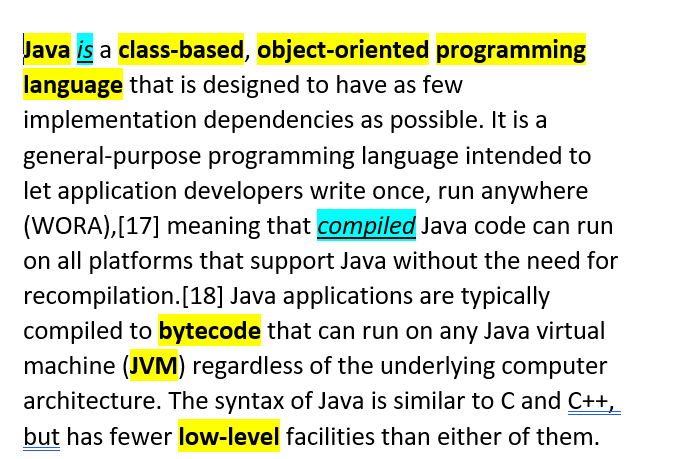
\includegraphics[scale=0.44]{initialdata.png}
	    \caption{A sample from the collated information}
	    \label{fig:wordfile}
	\end{figure}\\
	After defining the key terms in this document, they were added to a spreadsheet, where further analysis took place. For each individual term, a description was assigned by the domain expert, alongside the source of the term, the type of item it would become based on the colour codes from the previous step, and a final action that would define whether the term would progress to the lightweight ontology.
	\begin{figure}[h!]
	    \centering
	    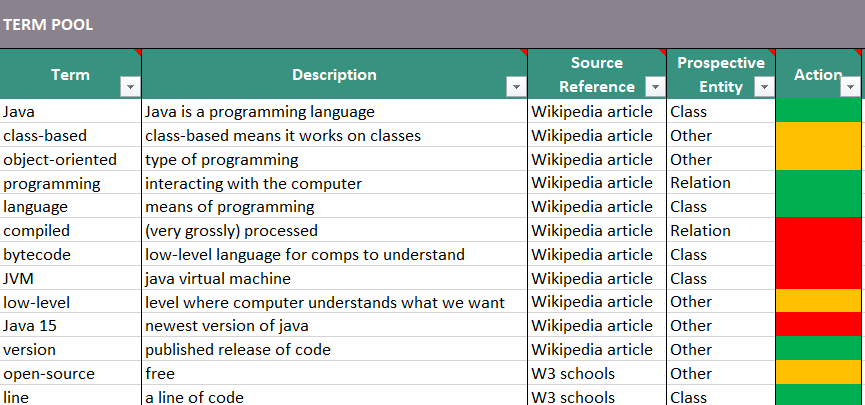
\includegraphics[scale = 0.65]{spreadsheet.png}
	    \caption{An extract of the Term Pool}
	    \label{fig:termpool}
	\end{figure}\\
	Following the final definition of the term pool, the lightweight ontology was created as a mind map, and later changed to a classic UML hierarchical representation.
	\subsection{Initial Structuring}
	With all the terms into place, the lightweight ontology could finally be created. By looking at all the classes available in the term pool that passed the progression test, the mind map took shape as below. The tool used to build this mind map is called Mural\cite{mural}.
	\begin{figure}[h!]
	    \centering
	    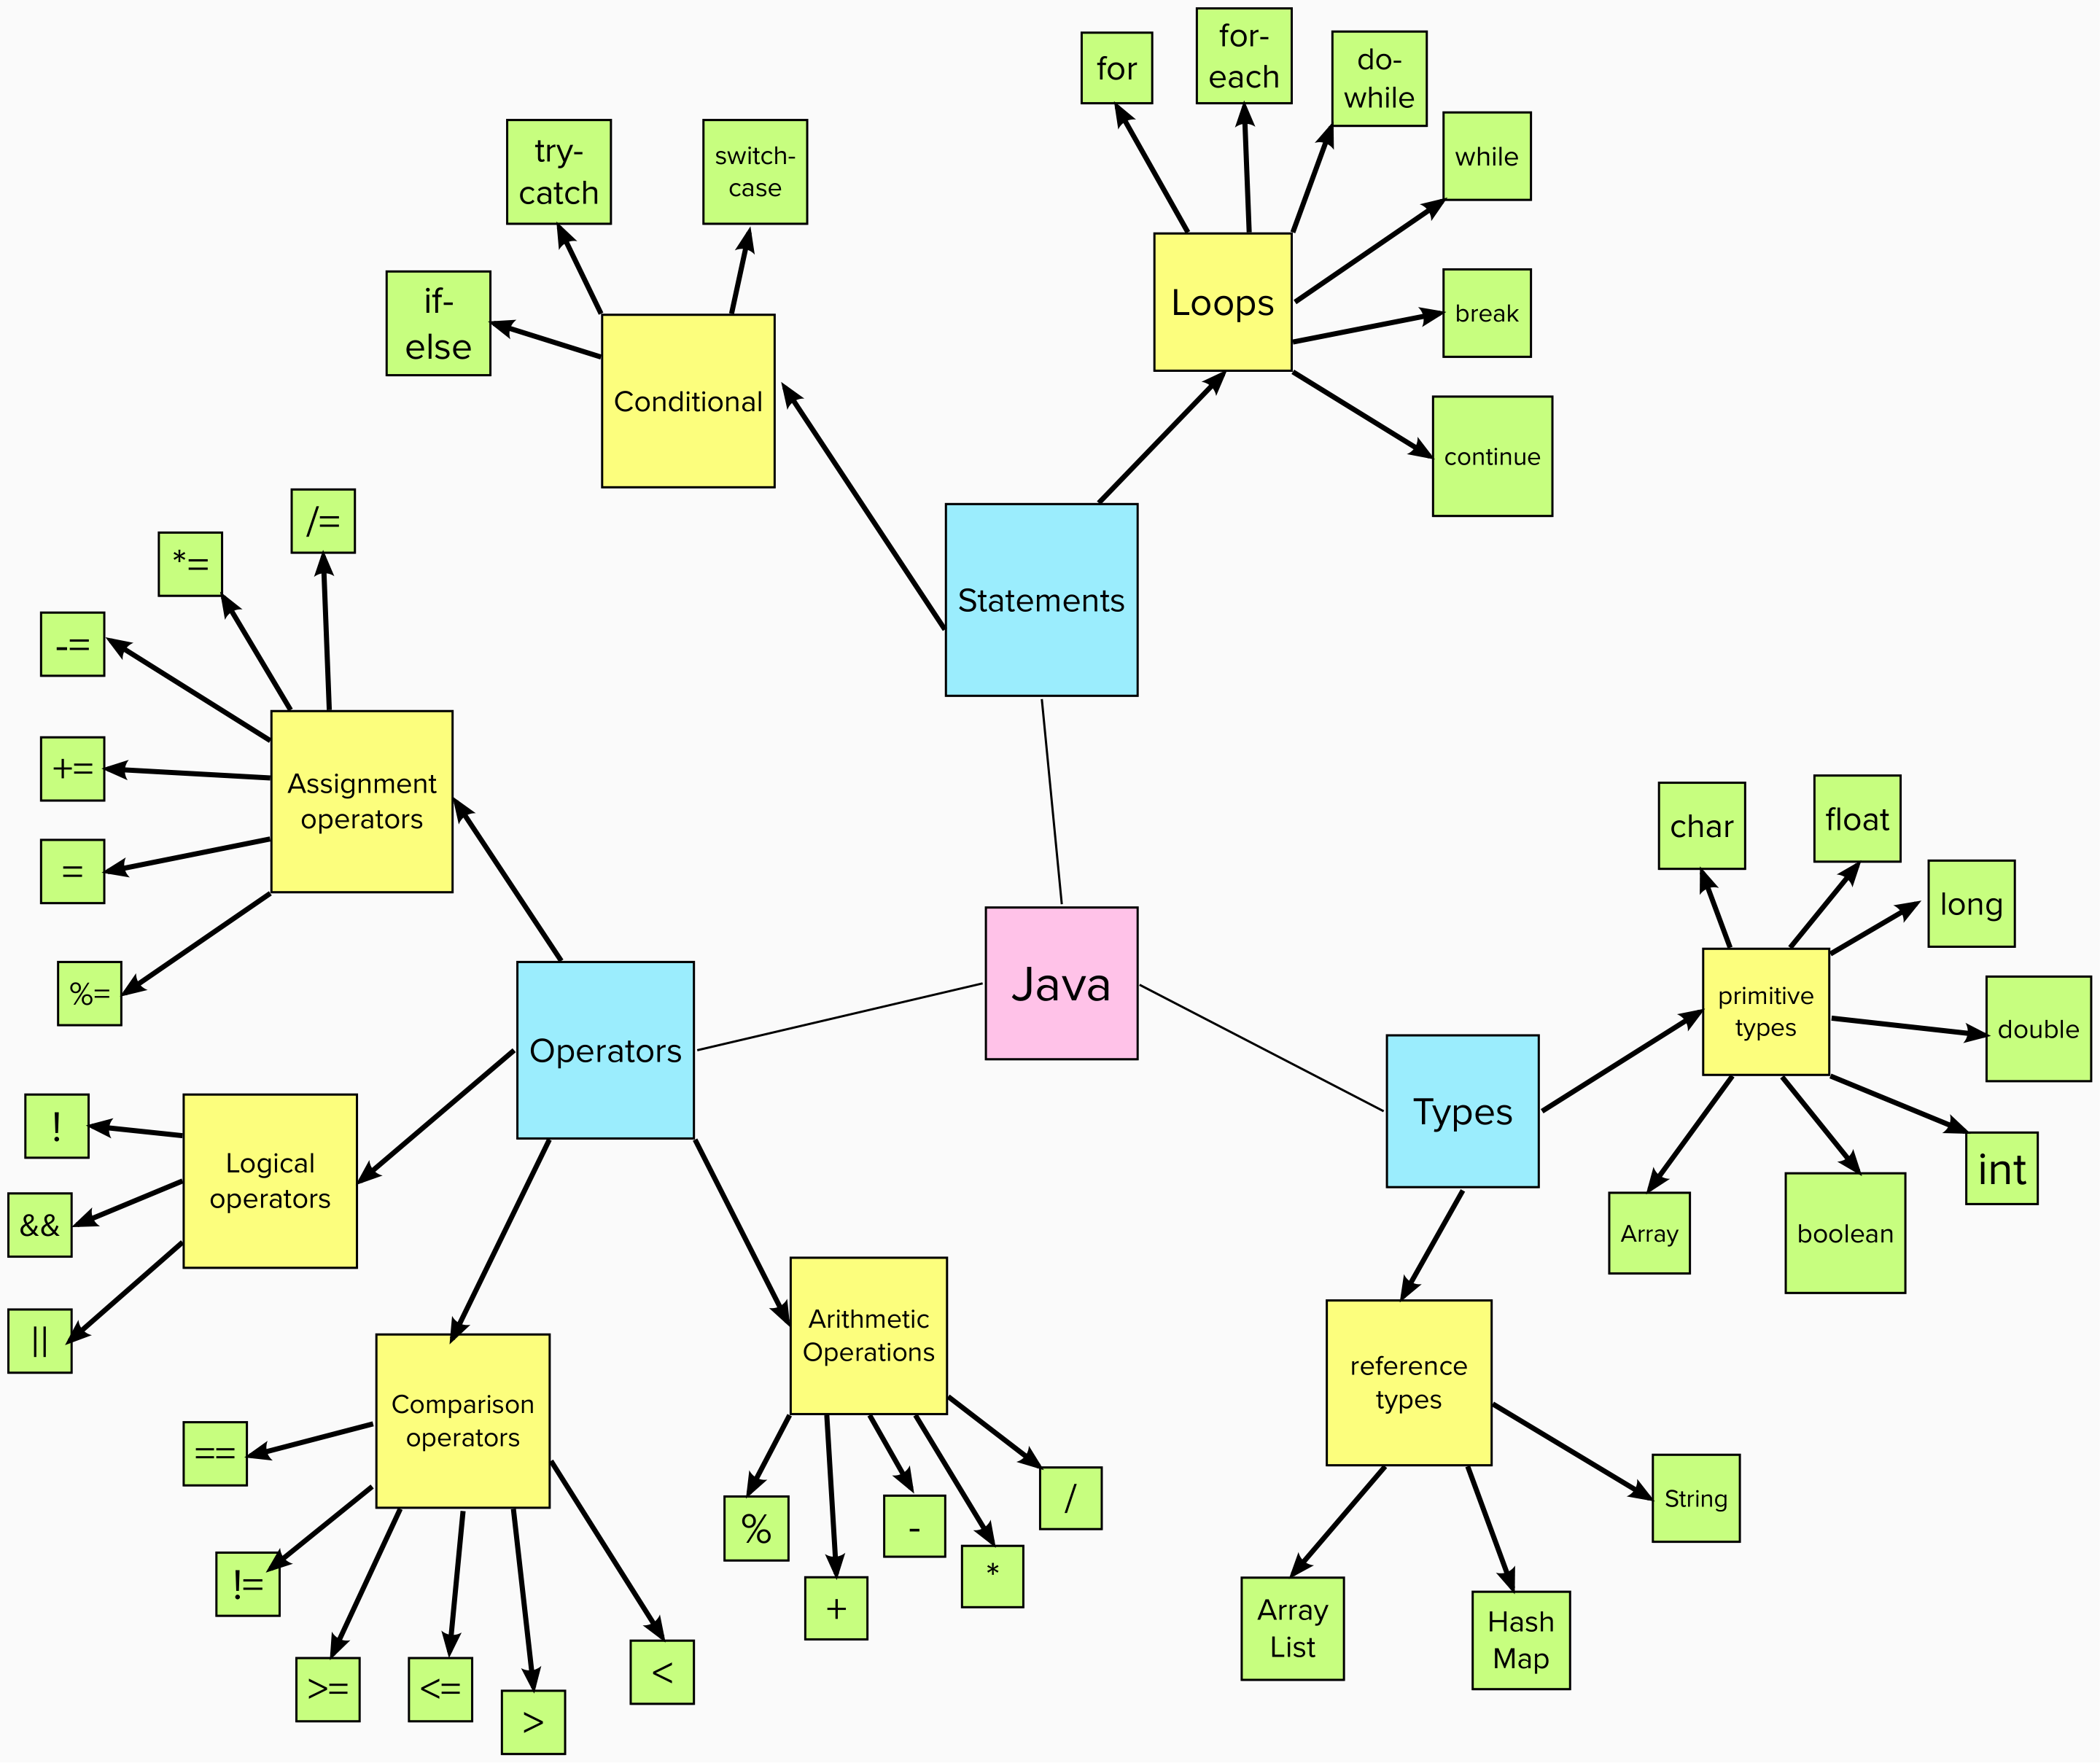
\includegraphics[scale = 0.13]{mindmap_new.png}
	    \caption{Initial Lightweight Ontology, the Mind Map}
	    \label{fig:mindmap}
	\end{figure}\\
	While this is a visually pleasing way to understand the hierarchical layers of the domain, it is not as descriptive as it should be in order to allow for ontology formalisation. It was a good and necessary intermediate step in order to understand how the lightweight ontology look like, but it perfectly illustrates the issue that semantic networks would have brought if formally implemented: lack of rigorousness.\\
	As the mind map was not informative enough, a different approach was taken to reconstruct the lightweight ontology. This came in the shape of a UML hierarchy, which is richer than the former representation. This new version also includes the relations between classes, as well as a small number of proposed instances for the heavyweight ontology.\\
	While not all the classes displayed in this visualisation made it to the final formalisation of the domain, the vast majority has been implemented. Moreover on top of the relations present in the UML, additional instances and relations were added.\\
	This visualisation marked the end of theoretical implementation, as it represents the stepping stone for the creation of the heavyweight ontology.
	
	\begin{figure}[h!]
	    \centering
	    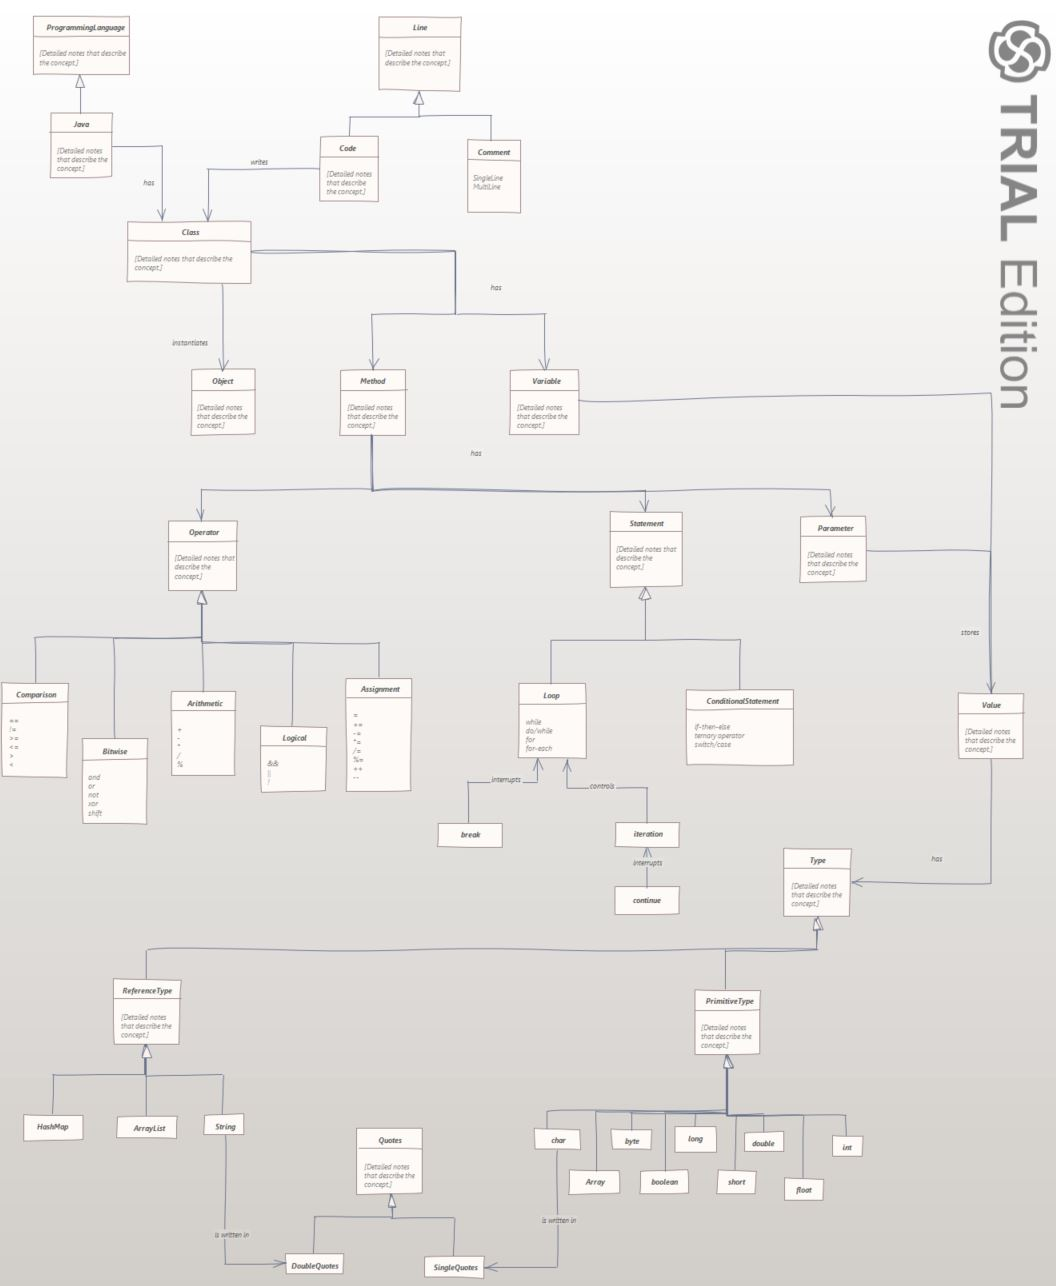
\includegraphics[width=\textwidth]{UML.JPG}
	    \caption{Second Lightweight Ontology: UML Representation}
	    \label{fig:uml}
	\end{figure}
	\clearpage
	
	\section{Ontology Formalisation}
	\section{Manipulating the Ontology with Apache Jena}
	\section{Front End Design}
	
	%Evaluation
	\chapter{Evaluation}
	
	%Conclusions and Future Work
	\chapter{Conclusions and Future Work}
	
	%Bibliography
	\begin{thebibliography}{99}
		\bibitem{itsdefinition} Intelligent Tutoring Systems, \href{https://en.wikipedia.org/wiki/Intelligent_tutoring_system}{Wikipedia.org}
		\bibitem{wikiontology} \href{https://en.wikipedia.org/wiki/Ontology_(information_science)}{Wikipedia.com}, Ontology (information science), Overview
        \bibitem{semnet} \href{https://www.obitko.com/tutorials/ontologies-semantic-web/semantic-networks.html}{obitko.com}, Ontologies and the Semantic Web, Semantic Networks
        \bibitem{semnetvsonto}Salem, Alfonse, 2008, Ontology versus Semantic Networks for Medical Knowledge
Representation, p 5
        \bibitem{rulesvsonto}Czarnecki \& Sitek, 2013, Ontologies vs. Rules — Comparison of Methods of Knowledge Representation Based on the Example of IT Services Management, p 108
        \bibitem{protege}\href{https://protege.stanford.edu/}{The Protégé website}
        \bibitem{protegerigin}\href{https://protege.stanford.edu/about.php}{The team behind Protégé}
        \bibitem{manchestersyntax}Horridge, Patel-Schneider, Manchester Syntax for OWL 1.1
        \bibitem{onto101}Noy, McGuinness, Ontology Development 101: A Guide to Creating Your First Ontology
        \bibitem{udemycourse} Chungoora, 2020, \href{Practical Knowledge Modelling: Ontology Development 101}{Practical Knowledge Modelling: Ontology Development 101}
        \bibitem{manchester} University of Manchester, 2011, A Practical Guide To Building OWL Ontologies Using Protégé 4 and CO-ODE Tools, Edition 1.3
        \bibitem{jena}\href{https://jena.apache.org/}{The Apache Jena website}
        \bibitem{tomcat}\href{http://tomcat.apache.org/}{The Apache Tomcat website}
        \bibitem{mural}\href{https://www.mural.co/}{Mural.co}

	\end{thebibliography}
	
	%Appendix
	\newpage
	\begin{center}
		\textbf{\large{Appendix}}
	\end{center}
	
	%User Guide
	\chapter{User Guide}
	
	%Program Listings
	\chapter{Program Listings}
	
\end{document}
